\documentclass[12pt]{article}

\usepackage[letterpaper, margin=1in]{geometry}
\usepackage{setspace}
\usepackage{parskip}
\usepackage{amsmath, amssymb}
\usepackage{booktabs}
\usepackage{graphicx}
\usepackage[authoryear,round]{natbib}
\usepackage{threeparttable}
\usepackage{longtable}
\usepackage{caption}
\usepackage{hyperref}
\hypersetup{hidelinks}

\defcitealias{sec2020}{SEC, 2020}

\doublespacing

\title{Pre-Mandate Human Capital Disclosure and the Information Content of Earnings: Evidence from Regulation S-K Item 101}
\author{Yeyang Zhou \\ John T. Steed School of Accounting \\ Price College of Business \\ University of Oklahoma}
\date{\today}

\begin{document}

\begin{titlepage}
\thispagestyle{empty}
\begin{singlespace}
\vspace*{1cm}
\begin{center}
{\Large\bfseries Pre-Mandate Human Capital Disclosure \\[0.2cm]
and the Information Content of Earnings: \\[0.2cm]
Evidence from Regulation S-K \par}
\vspace{0.9cm}
{\large Yeyang Zhou \par}
\vspace{0.3cm}
{\small John T. Steed School of Accounting \\
Price College of Business \\
University of Oklahoma \par}
\vspace{0.5cm}
{\small\today}
\end{center}

\vspace{1.0cm}

\begin{center}{\textbf{Abstract}}\end{center}
\vspace{-0.2cm}
{
\noindent This paper examines whether firms with different levels of pre-mandate human capital disclosure (HCD) intensity experienced different changes in earnings response coefficients (ERC) following the SEC's 2020 Regulation S-K Item 101 amendment. Using a triple-interaction design with 17{,}544 firm-year observations from U.S. firms over 2017 to 2023, I find that the coefficient on $Post \times HCD \times UE$ is not statistically significant. This null finding suggests that firms with higher pre-mandate HCD intensity did not experience a differential post-mandate change in the earnings-return relation. 
\par\vspace{0.4cm}
\noindent\textbf{Keywords:} Earnings response coefficient; Human capital disclosure; Regulation S-K; Mandatory disclosure
}

\vfill
\end{singlespace}
\end{titlepage}


\section{Introduction}

This paper examines whether mandatory human capital disclosure changes how investors respond to earnings news. Specifically, I use the SEC's 2020 Regulation S-K Item 101 amendment as a regulatory shock to firms' human capital disclosure environment. I investigate whether firms with different levels of pre-mandate human capital disclosure (HCD) intensity experience different changes in earnings response coefficients (ERC) after the mandate.

Human capital has become an important value driver for many firms. Employees, training, retention, organizational knowledge, and workforce stability can affect firms' future cash flows. However, traditional financial statements do not fully capture many human capital investments. For example, training and employee development are often expensed rather than recognized as assets. As a result, investors may observe the earnings number but still have limited information about the workforce conditions behind that earnings number.

The Regulation S-K Item 101 Amendment took effect on November 9, 2020. The U.S. Securities and Exchange Commission (SEC) required registrants to disclose a description of their material human capital resources, including measures or objectives the firm focuses on in running the business \citepalias{sec2020}.

The final rule explicitly justified the amendment on the ground that human capital is often a material resource and an important driver of performance, and it adopted a principles-based design rather than a fixed metric set. The registrants have the discretion to report human capital measures and objectives such as measures or objectives that address the attraction, development, and retention of personnel.



% There are many cross-sectional variations in the human capital disclosure by firms. I have three examples of low, middle, and high human capital disclosure in the Appendix.

Before the amendment, Item~101 required only a checklist-style disclosure of the number of persons employed by the firm at fiscal year-end. After the amendment, Item~101(c) requires firms to disclose, on a principles-based basis, a description of their human capital resources, including any human capital measures or objectives that management focuses on in operating the business, such as those addressing the development, attraction, and retention of personnel. The disclosure is mandatory and is filed as part of the firm's 10-K. Early evidence shows that firms did increase human capital disclosure \citep{bourveau_al2022} after the amendment, yet the resulting disclosures remained highly heterogeneous and often not comparable within industries. 

{Using a sample of 17{,}544 firm-year observations from 3{,}248 U.S. firms over fiscal years 2017 to 2023, I find that the differential change in ERC following the mandate is not statistically distinguishable from zero. This null finding indicates that firms with different pre-mandate HCD intensity did not experience a differential post-mandate change in the earnings-return relation.}

{This paper contributes to the literature on the capital market effects of mandatory disclosure regulation. Prior work documents that the SEC's 2020 HCD mandate generated filing-date market reactions, shifted the topics and language of human capital disclosure, and is associated with workforce outcomes such as employee turnover. This paper examines a related but distinct question: whether the earnings-return relation itself shifted differentially across firms with different prior disclosure environments. The null finding for the change-of-earnings specification provides evidence on the empirical limits of inferring a disclosure-quality channel from pre-mandate exposure measures.}

\section{Literature Review}

\subsection{Earnings Response Coefficient}

The earnings response coefficient (ERC) measures how strongly stock prices respond to unexpected earnings. A larger ERC means that investors view the earnings innovation/surprise as more informative. The earnings response coefficient literature begins with \citet{ballBrown1968}. They show that the sign of unexpected earnings can predict the direction of stock returns around the earnings announcement. This finding establishes that accounting earnings have information content, and reveals the relation between earnings and returns, but the magnitude of how returns respond to earnings remains unexplored.

Prior ERC research shows that this response is not identical for all the firms. The same earnings surprise can generate a large market reaction for one firm but a small reaction for another firm. \citet{collinsKothari1989} study the cross-sectional and time-series determinants of ERC, and document that ERC are affected by riskless interest rates, the riskiness, growth and persistence of earnings. Specifically, the coefficient is increasing in the persistence of the earnings innovation, decreasing in the riskiness of the firm and the discount rate, and increasing in the precision with which the market is able to interpret the reported earnings number.

For this study, I organize these determinants into a three-part valuation framework. An earnings innovation should have a larger ERC when it leads investors to revise expected future cash flows more strongly, when those expected cash flows are discounted at a lower rate, and when investors can interpret the earnings signal more precisely.

\subsubsection{Earnings persistence}

The first valuation component is expected future cash flows. In the ERC literature, current earnings news is important because it helps investors update beliefs about future earnings and future cash flows. \citet{collinsKothari1989} show that ERC is higher when earnings innovations are more persistent. The reason is simple. If an earnings shock is expected to continue into the future, then it affects many future periods, not just the current year. Investors should therefore place a larger value weight on that earnings surprise.

\subsubsection{Discount rates and information risk}

The second valuation component is the discount rate. \citet{collinsKothari1989} argue that ERC is lower when firm risk or the expected rate of return is higher. This is because future cash-flow revisions are worth less when they are discounted at a higher rate. \citet{eastonZmijewski1989} make a related point: the earnings response is weaker when investors require a higher expected return.

Disclosure theory provides a direct link between information and discount rates. \citet{lambert_al2007} show that accounting information quality can affect the cost of capital. Better information can reduce uncertainty about future cash flows. It can also affect investors' assessment of risk. Therefore, disclosure may increase ERC not only by changing expected future cash flows, but also by changing the rate used to discount those cash flows.

\subsubsection{Precision in mapping earnings into value}

The third valuation component is precision. ERC should be higher when investors can interpret earnings news more precisely. \citet{holthausenVerrecchia1988} show that market reactions depend on the precision of information signals and the information environment surrounding the announcement. \citet{verrecchia2001} also emphasizes that disclosure affects capital markets by changing information asymmetry and the way information is incorporated into prices.

This precision component is central to my setting because HCD can change how investors interpret earnings innovations. Earnings are an aggregate number, and they combine many economic forces. Without additional information, investors may not know whether strong earnings come from durable labor productivity, temporary cost cutting, weak investment in employees, or favorable short-term conditions.

However, the effect of HCD depends on whether the disclosure provides incremental information. If HCD adds useful context, it may help investors understand what current earnings imply for future performance. If similar information was already available before the mandate, the incremental effect of the new disclosure may be limited. Therefore, the relation between mandatory HCD and ERC depends not only on whether firms disclose more human capital information after the mandate, but also on how much useful information investors already had before the mandate.

\subsection{Disclosure Regulation and Capital Market Effects}

Disclosure regulation can affect capital markets by changing the information available to investors. \citet{verrecchia2001} provides a broad framework for understanding disclosure through information asymmetry, managerial discretion, and market efficiency. In this framework, disclosure matters because it can reduce uncertainty and help investors form better beliefs about firm value.

Mandatory disclosure is important when voluntary disclosure is incomplete. Managers may not fully disclose information if it is costly, proprietary, difficult to verify, or unfavorable. Regulation can force firms to provide information that investors may find useful but that managers may otherwise disclose selectively. However, mandatory disclosure does not automatically improve market outcomes. The effect depends on whether the disclosure is credible, useful, and processed by investors.

Prior research shows that mandatory disclosure can improve liquidity, reduce information asymmetry, and increase the information content of announcements. These effects are often stronger when firms had weaker information environments before the regulation. This point is important for my setting because the SEC's 2020 HCD rule may have different effects depending on firms' pre-mandate disclosure environments.

On the one hand, firms with low pre-mandate HCD may experience larger information improvements because they had larger disclosure gaps before the mandate. For these firms, the rule may provide investors with new information about human capital resources, workforce risks, and labor strategy. This can improve investors' ability to interpret earnings news.

On the other hand, firms with high pre-mandate HCD may also experience larger effects if prior disclosure intensity reflects stronger disclosure capability and a greater commitment to human capital communication. These firms may be better prepared to provide specific and decision-useful disclosure after the mandate. Investors may also view their post-mandate HCD as more credible because these firms had already discussed human capital before the rule.

\subsection{Human Capital Disclosure: Empirical Evidence}

Human capital disclosure is a useful setting for studying whether nonfinancial disclosure helps investors interpret earnings. Human capital is an important input into firm performance, but it is not fully captured by traditional financial statements. Many human capital investments, such as training, employee development, retention, and organizational knowledge, are expensed or not separately recognized as assets. Therefore, investors may know the earnings number, but they may not fully understand the human capital conditions behind that earnings number. HCD can help fill this gap by providing information about the workforce, labor strategy, employee development, and retention.

Prior research suggests that HCD contains economically meaningful information. \citet{arif_al2022} examine the information content of newly mandated qualitative HCD for equity and bond investors. They find that the amount of HCD is negatively associated with contemporaneous employee turnover. They also document that both total and unexpected HCD generate positive equity market reactions around the 10-K filing date. Their evidence suggests that mandatory HCD is not pure boilerplate. It contains information that investors use when they update beliefs about firm value.

Other studies also show that HCD reflects real workforce conditions. \citet{dey_al2025} examine turnover disclosures using a proprietary dataset of more than 8.6 million career histories and textual analysis of SEC filings. They find that firms adjust the intensity and tone of turnover disclosures in response to changes in employee flows. This relation is stronger for firms with more high-skilled employees. Their findings suggest that turnover-related disclosure responds to actual labor dynamics. This evidence is important for my study because employee turnover and workforce stability can affect the persistence of earnings. If HCD helps investors understand whether current earnings are supported by a stable workforce, then HCD may also help investors interpret earnings news.

A related stream of research examines how firms changed their HCD after the SEC's 2020 Regulation S-K amendment. \citet{bourveau_al2022} study the evolution of HC disclosures by U.S. public firms from 2017 to 2024. Using 10-K filings, sustainability reports, and EEO-1 disclosures, they document a significant increase in HC disclosures, especially disclosures related to diversity, equity, and inclusion (DEI) and turnover. They also find that firms are more likely to disclose metrics in 10-Ks when they previously disclosed related information voluntarily. This suggests that firms consider topic-specific costs and benefits when deciding what human capital information to disclose. Their evidence is useful because it shows that the mandate increased HCD, but not in a uniform way.

The non-uniform nature of HCD is important. The 2020 rule is principles-based. It requires firms to disclose material human capital information, but it does not require a fixed set of metrics. As a result, firms differ in the topics, specificity, and quantitative detail of their disclosures. This creates both an opportunity and a challenge. The opportunity is that the mandate increased the availability of human capital information in 10-K filings. The challenge is that the information may not be equally useful across firms. Some firms may provide specific and decision-useful disclosure, while others may provide general language.

\citet{mayewZhang2024} provide evidence that HCD can matter for valuation in a more specific setting. They study corporate human capital management responses to the COVID-19 pandemic. Using mandated SEC human capital disclosures in 10-K filings to measure COVID-related HCM investments, they find that favorable valuation effects appear only when financial flexibility is higher. This finding is important because it suggests that human capital investment is not always valued positively by the market. Investors appear to consider whether firms have enough resources to support those investments. This supports a conditional view of HCD. Human capital information may be value relevant, but its valuation effect depends on the firm's economic context.

\citet{zhang2022} studies HCM disclosure transparency using a word embedding model. The study finds that when product market competition is high, firms disclose more social-oriented HCM information but less operational-oriented HCM information. This evidence is also useful for my setting because it shows that HCD is shaped by firms' disclosure incentives. Managers may disclose some types of human capital information more readily than others. Operational human capital information may be more proprietary or more costly to reveal. Therefore, HCD quality and content are likely endogenous to firm incentives and competitive conditions. This reinforces the need to examine not only whether firms disclose more HCD, but also whether the disclosure improves investors' interpretation of earnings.

However, this literature has not directly examined whether mandatory HCD changes the earnings-return relation. Prior studies mainly focus on filing-date reactions, disclosure quantity, disclosure topics, valuation effects, turnover disclosure, and labor-market outcomes. These are important outcomes, but they do not show whether HCD changes how investors respond to earnings news. This is the gap my study addresses.

More importantly, my setting does not only ask whether the mandate changed ERC on average. My research design examines whether firms with different pre-mandate HCD intensity experienced different changes in the market response to earnings innovations after the SEC's 2020 mandate. This distinction is important because pre-mandate HCD intensity can capture two different economic forces. It may capture better disclosure capability and preparation for the mandate. It may also capture a more saturated pre-mandate information environment, where the mandate adds less incremental information. Therefore, the expected relation between pre-mandate HCD intensity and post-mandate changes in ERC is theoretically ambiguous.

\section{Hypothesis Development}

The literature review suggests that human capital disclosure can affect the information environment around earnings. However, my research design does not estimate the average effect of the SEC's 2020 human capital disclosure mandate on ERC. Instead, it examines whether firms with different levels of pre-mandate HCD intensity experienced different changes in ERC after the mandate.

This distinction is important. The treatment-exposure variable in this study is firm-level pre-mandate HCD intensity, measured over FY2015--FY2019 using the \citet{demers_al2024} lexicon applied to Item 1 of 10-K filings. Therefore, the main empirical coefficient does not capture whether mandatory HCD increased ERC for the average firm. Rather, it captures whether the change in ERC from the pre-mandate to the post-mandate period differs between firms with higher and lower pre-mandate HCD intensity.

There are two competing forces. They predict different signs for the relation between pre-mandate HCD intensity and post-mandate changes in ERC.

The first force is a disclosure-quality or preparation-advantage mechanism. Firms with higher pre-mandate HCD intensity may already have stronger internal systems for collecting, organizing, and communicating human capital information. They may also have managers who are more committed to human capital communication. When the SEC mandate makes HCD part of required 10-K disclosure, these firms may be better prepared to provide more specific and decision-useful information. Investors may also view their disclosures as more credible because these firms had already discussed human capital before the mandate.

Under this mechanism, high pre-mandate HCD intensity predicts a stronger post-mandate improvement in the earnings information environment. These firms may provide HCD that helps investors interpret earnings more effectively. The disclosure may help investors assess whether current earnings are supported by stable employees, training, retention, workforce productivity, or other human capital fundamentals. It may also help investors understand labor-related risks and the growth implications of earnings. As a result, earnings news becomes more informative for valuation. This force predicts that ERC increases more after the mandate for firms with higher pre-mandate HCD intensity.

The second force is an information-substitution or saturation mechanism. Firms with higher pre-mandate HCD intensity may have already provided substantial human capital information before the SEC mandate. For these firms, investors may have already incorporated much of the relevant labor-related information into their valuation process. In that case, the mandate may add little incremental information. The post-mandate disclosure may formalize or slightly expand information that investors already had, but it may not substantially change how investors interpret earnings.

By contrast, firms with lower pre-mandate HCD intensity had larger pre-mandate information gaps. Investors likely had less information about their workforce, labor strategy, employee retention, and human capital risks before the mandate. For these firms, the mandatory disclosure requirement may create a larger improvement in the information environment. Even if their post-mandate HCD is not perfect, the new disclosure may provide information that was previously unavailable. As a result, investors may become better able to interpret earnings for firms that were previously less transparent about human capital. This force predicts that ERC increases more after the mandate for firms with lower pre-mandate HCD intensity.

These two mechanisms lead to opposite predictions for the main coefficient. If the disclosure-quality or preparation-advantage mechanism dominates, the coefficient on the interaction of Post, pre-mandate HCD intensity, and unexpected earnings should be positive. This would suggest that firms with higher pre-mandate HCD intensity experienced a larger post-mandate increase in ERC. If the information-substitution or saturation mechanism dominates, the coefficient should be negative. This would suggest that firms with lower pre-mandate HCD intensity experienced a larger post-mandate increase in ERC because they benefited more from the new disclosure requirement.

Therefore, the sign of the main coefficient is an empirical question. The mandate may improve the earnings information environment more for firms that were already prepared to disclose high-quality human capital information. Or it may improve the earnings information environment more for firms that previously disclosed little human capital information and had larger information gaps. My empirical test is designed to distinguish between these two forces.

Accordingly, I state the hypothesis in non-directional form:

\medskip
\noindent\textbf{H1:} \textit{The change in ERC after the SEC's 2020 human capital disclosure mandate differs systematically with firms' pre-mandate human capital disclosure intensity.}
\medskip

\section{Data}

I construct a firm-year panel using Compustat, CRSP, and human capital disclosure data. The sample period covers fiscal years 2015 to 2024. The pre-mandate period is FY2015--FY2019, and the post-mandate period begins in FY2020, following the effective date of the SEC's Regulation S-K Item 101 amendment in November 2020.

Financial statement data come from Compustat annual fundamentals. I use Compustat to obtain earnings, total assets, shares outstanding, stock price, fiscal year-end date, and industry classification. I apply standard Compustat filters and keep industrial format, standard data format, domestic population source, and consolidated statements. I exclude financial firms and utilities because these industries have different reporting environments, regulatory structures, and valuation models.

Stock return data come from CRSP monthly stock files. I link Compustat firms to CRSP securities using the CRSP/Compustat Merged link table. I keep common U.S. equity securities and require valid monthly returns. I also use the CRSP value-weighted market return to construct market-adjusted buy-and-hold returns.

After applying the sample restrictions (non-missing earnings, total assets, market value, and lagged scalers; valid CRSP links and monthly returns; pre-mandate HCD exposure measured over FY2015--FY2019; all four unexpected earnings measures non-missing; and the $\pm 3$-year window around the FY2020 post-mandate cutoff), the final regression sample consists of 17,544 firm-years from 3,248 unique firms over FY2017--FY2023. All continuous variables are winsorized at the 1st and 99th percentiles, and standard errors are clustered by firm in all regressions. Table~\ref{tab:sample} in the Appendix reports the full sample selection.

\section{Methods}

\subsection{Measure}

The complete set of variables used in the analysis is defined in Table~\ref{tab:vardef} in the Appendix. The remainder of this subsection describes the construction of the key variables in more detail.

\subsubsection{Pre-Mandate Human Capital Disclosure Intensity}

The main treatment-exposure variable is pre-mandate human capital disclosure intensity. I measure this variable at the firm level using human capital disclosure in 10-K Item 1 before the SEC mandate. Specifically, I use the \citet{demers_al2024} human capital disclosure lexicon and apply it to Item 1 text in firms' 10-K filings from FY2015 to FY2019.

For each firm-year in the pre-mandate period, I measure the intensity of human capital disclosure based on the frequency of human capital terms in Item 1. I then average this measure across FY2015--FY2019 to obtain a firm-level pre-mandate HCD intensity measure. This measure is time-invariant in the main analysis. I standardize it to have a mean of zero and a standard deviation of one. I refer to the standardized measure as HCD.

This variable captures firms' exposure to the 2020 HCD mandate. It does not measure post-mandate disclosure directly. This distinction is important. A higher value of HCD means that the firm had more intensive human capital disclosure before the mandate. In the empirical design, I use this pre-mandate measure to test whether firms with different prior HCD intensity experienced different changes in ERC after the SEC rule became effective.

\subsubsection{Return Measure}

The dependent variable is cumulative stock return around the fiscal year-end earnings period. I construct buy-and-hold returns using CRSP monthly returns. The return measure used throughout the empirical analysis is the market-adjusted buy-and-hold return over the window from eight months before fiscal year-end to three months after fiscal year-end. I refer to this measure as \textit{BHRetMktm9p3}. This return window is designed to capture the market response to annual earnings information while allowing for the timing of annual report filing and earnings-related information release. Market-adjusted returns are calculated by subtracting the CRSP value-weighted market return from the firm's monthly return before compounding. 
% This adjustment helps remove broad market-wide return movements that are unrelated to firm-specific earnings news.

\subsubsection{Unexpected Earnings Measures}

The key earnings variable is unexpected earnings. In the main analysis, I use the change in income before extraordinary items scaled by lagged market value of equity ($c1IB\_L1MV$). This specification follows a random-walk model of expected earnings: the prior year's earnings serve as the implicit benchmark, and the year-over-year change in earnings, scaled by lagged market value of equity, proxies for the earnings surprise. Market value of equity is measured as shares outstanding multiplied by fiscal year-end stock price. Lagged market value is based on the prior fiscal year. Scaling earnings by lagged market value helps make the earnings measure comparable across firms.

I also construct three alternative unexpected earnings measures, all of which are reported alongside the main measure in the empirical tables. First, $IB\_L1MV$ is the level of income before extraordinary items scaled by lagged market value of equity; this corresponds to the earnings-yield specification of the ERC and is reported as an alternative because the level and change specifications carry different implicit assumptions about expected earnings. Second, $c1IB\_L1P$ is the change in earnings per share scaled by lagged stock price. Third, $c1IB\_L1TA$ is the change in income before extraordinary items scaled by lagged total assets.

Using multiple unexpected earnings measures is useful because ERC estimates can be sensitive to how unexpected earnings are measured. The main tests report results for all four measures.

\subsection{Model}

I estimate the following firm-year panel regression to test H1:
\begin{equation}
\begin{aligned}
AR_{i,t} \;=\;& \alpha + \beta_1\, UE_{i,t} + \beta_2\, (Post_t \times UE_{i,t}) + \beta_3\, (HCD_i \times UE_{i,t}) \\
&+ \beta_4\, (Post_t \times HCD_i) + \beta_5\, (Post_t \times HCD_i \times UE_{i,t}) + \mu_i + \lambda_t + \varepsilon_{i,t}
\end{aligned}
\label{eq:main}
\end{equation}

\noindent where $AR_{i,t}$ is firm $i$'s buy-and-hold return over the fiscal-year-end return window (market-adjusted in the main specification); $UE_{i,t}$ is unexpected earnings (change in income before extraordinary items scaled by lagged market value of equity in the main specification); $HCD_i$ is the firm-level pre-mandate HCD intensity measure (FY2015--FY2019 average, standardized); and $Post_t$ equals one for fiscal years on or after the post-mandate cutoff and zero otherwise. The model includes firm fixed effects ($\mu_i$) and year fixed effects ($\lambda_t$). Standard errors are clustered by firm.

The coefficients have the following interpretations. $\beta_1$ captures the baseline ERC in the pre-mandate period. $\beta_2$ captures the average post-mandate shift in ERC across all firms. $\beta_3$ captures the pre-mandate relation between HCD intensity and ERC and serves as a control. $\beta_4$ captures the direct effect of pre-mandate HCD intensity on returns in the post-mandate period and is also a control. The focal coefficient is $\beta_5$, which captures the differential change in ERC after the mandate between firms with higher and lower pre-mandate HCD intensity.

The main effects of $Post_t$ and $HCD_i$ do not appear in equation~(\ref{eq:main}) because they are absorbed by the year fixed effects and firm fixed effects, respectively. The interaction term $Post_t \times HCD_i$ varies at the firm-year level and is not absorbed by the fixed effects, so it is included explicitly to obtain unbiased estimates of $\beta_5$.

Under H1, $\beta_5$ is non-zero. A positive $\beta_5$ is consistent with the disclosure-quality or preparation-advantage mechanism, while a negative $\beta_5$ is consistent with the information-substitution or saturation mechanism. I also estimate a baseline ERC specification that omits the $HCD$ interactions to assess whether the mandate is associated with an average change in ERC.

{\section{Results}

\subsection{Sample and Descriptive Statistics}

Table~\ref{tab:desc} reports descriptive statistics for the main variables in the regression sample after winsorization at the 1st and 99th percentiles. The market-adjusted buy-and-hold return ($BHRetMktm9p3$) has a mean of $-0.028$ and a median of $-0.104$, consistent with the negative skewness of long-horizon returns. The main unexpected earnings measure, $c1IB\_L1MV$, has a mean of $0.021$ and a median of $0.002$, indicating a roughly symmetric distribution centered near zero, as would be expected of an earnings-change variable. The standardized pre-mandate HCD intensity measure ($HCD$) has a mean of $0.085$ and a standard deviation of $1.004$ within the regression subsample.

\subsection{Main ERC Regression}

Table~\ref{tab:main} reports the main ERC regression results. The dependent variable is the market-adjusted buy-and-hold return around the fiscal year-end earnings period. The main variable of interest is the triple interaction term, $Post \times HCD \times UE$. This coefficient tests whether firms with higher pre-mandate HCD intensity experienced a different change in ERC after the SEC mandate.

Column (1) is my main specification. In this column, unexpected earnings are measured as the change in income before extraordinary items scaled by lagged market value of equity. The coefficient on $Post \times HCD \times UE$ is $-0.027$, and it is not statistically significant. This means that I do not find evidence that firms with higher pre-mandate HCD intensity had a different post-mandate change in the earnings-return relation.

The coefficient on $UE$ is positive and significant in Column (1). This suggests that, before the mandate, earnings changes were positively associated with stock returns. The coefficient on $Post \times UE$ is also positive and marginally significant, suggesting that the average ERC may have increased after the mandate. However, the key result is that this increase does not appear to differ systematically with pre-mandate HCD intensity.

Columns (2) to (4) use alternative measures of unexpected earnings. The results are mixed. The change-in-EPS measure gives a similar insignificant result. The assets-scaled earnings-change measure is only marginally significant. The earnings-yield measure is positive and significant. However, the earnings-yield measure is a level measure, while the main test uses an earnings-change measure to proxy for earnings surprises. Therefore, I treat the earnings-change specification as the main result.

Overall, Table~\ref{tab:main} provides limited support for the hypothesis. The main specification does not show that pre-mandate HCD intensity predicts differential changes in ERC after the SEC mandate.

\subsection{Robustness}

Table~\ref{tab:robust} examines whether the main result is sensitive to sample and research design choices. I vary two choices. First, I change the post-mandate cutoff from FY2020 to FY2021. Second, I compare a $\pm 3$-year window with a $\pm 5$-year window. I also repeat the tests after excluding FY2020 because FY2020 overlaps with both COVID-19 and the transition into the new disclosure rule.

The results for the main unexpected earnings measure are generally weak. When unexpected earnings are measured as the change in income scaled by lagged market value, the coefficient on $Post \times HCD \times UE$ is negative across the specifications. Some estimates are marginally significant, but the overall pattern is not strong enough to support a clear conclusion.

The results are also not consistent across the alternative earnings measures. The change-in-EPS measure is mostly insignificant. The assets-scaled earnings-change measure changes sign across specifications. The earnings-yield measure is positive and significant in several columns, but this measure captures a different concept from the earnings-change measures.

Overall, the robustness tests do not provide strong evidence that pre-mandate HCD intensity is associated with a differential change in ERC after the mandate. The main conclusion remains the same: using the earnings-change measure as the main proxy for unexpected earnings, I do not find a statistically reliable HCD-related change in the earnings-return relation.}


\section{Conclusion}

This paper examines whether firms with different levels of pre-mandate human capital disclosure (HCD) intensity experienced different changes in earnings response coefficients (ERC) after the SEC's 2020 Regulation S-K Item 101 amendment. Using a firm-year panel of 17,544 observations from 3,248 U.S. firms over FY2017--FY2023, I estimate a triple-interaction specification that compares the pre- to post-mandate change in the earnings-return relation across firms with different pre-mandate HCD intensity. The pre-mandate exposure measure is the firm-level average of Item~1 HCD intensity over FY2015--FY2019, constructed using the \citet{demers_al2024} lexicon.

The main result is a null finding. In the main specification, where unexpected earnings are measured as the change in income before extraordinary items scaled by lagged market value of equity, the coefficient on $Post \times HCD \times UE$ is $-0.027$ and not statistically distinguishable from zero. Robustness tests that vary the post-mandate cutoff (FY2020 versus FY2021), the estimation window ($\pm 3$ versus $\pm 5$ fiscal years), and the inclusion of FY2020 do not yield a consistent pattern. Alternative unexpected earnings measures generate mixed signs and significance, but the change-based main specification remains insignificant across cuts of the data.

This null finding has two implications. First, it does not imply that mandatory HCD is uninformative. Prior work documents filing-date market reactions, shifts in disclosure topics, and labor-market consequences of the mandate. The null result here speaks to a narrower question: whether pre-mandate HCD intensity, as a measure of firms' prior disclosure capability or saturation, predicts a differential change in how investors translate earnings news into prices. The data do not support that prediction.

Second, the result highlights the difficulty of inferring a disclosure-quality channel from pre-mandate exposure alone. The two competing mechanisms developed in the hypothesis---a preparation-advantage channel and an information-substitution channel---offer opposite predictions, and the design used here cannot separate them when their net effect is small. Future work could measure post-mandate HCD specificity directly, examine within-industry variation, or use textual measures that capture the informativeness rather than the volume of disclosure. These extensions may have more power to detect a disclosure-quality channel in the earnings-return relation than the pre-mandate intensity measure used in this paper.




\clearpage
\bibliographystyle{plainnat}
\bibliography{References_Zhou}

\clearpage

\begin{table}[ht]
\centering
\caption{Descriptive Statistics}
\label{tab:desc}
\small
\begin{threeparttable}
\begin{tabular}{lrrrrrrr}
\toprule
\textbf{Variable} & \textbf{N} & \textbf{Mean} & \textbf{Std.} & \textbf{P25} & \textbf{Median} & \textbf{P75} & \textbf{Max} \\
\midrule
$BHRetMktm9p3$    & 17{,}544 & $-$0.0276 & 0.5742 & $-$0.3695 & $-$0.1043 & 0.1742 & 2.3425 \\
$c1IB\_L1MV$      & 17{,}544 &  0.0214 & 0.3873 & $-$0.0381 &  0.0016 & 0.0369 & 3.0903 \\
$IB\_L1MV$        & 17{,}544 & $-$0.1211 & 0.4450 & $-$0.1307 &  0.0107 & 0.0528 & 0.6264 \\
$c1IB\_L1P$       & 17{,}544 & $-$0.0233 & 0.6037 & $-$0.0307 &  0.0036 & 0.0433 & 3.4335 \\
$c1IB\_L1TA$      & 17{,}544 & $-$0.0048 & 0.3085 & $-$0.0501 &  0.0025 & 0.0451 & 2.2076 \\
$HCD$ (std.)      & 17{,}544 &  0.0851 & 1.0037 & $-$0.5393 & $-$0.0755 & 0.4225 & 8.3044 \\
$HCD$ (raw)       & 17{,}544 &  0.0113 & 0.0066 &  0.0072 &  0.0102 & 0.0135 & 0.0655 \\
\bottomrule
\end{tabular}
\begin{tablenotes}
\footnotesize
\item Notes: Descriptive statistics for the final regression sample of 17,544 firm-years from 3,248 unique firms over fiscal years FY2017--FY2023, formed by intersecting the pre-period HCD-matched panel with the requirement that the main dependent variable ($BHRetMktm9p3$) and all four unexpected earnings measures be non-missing, and that fiscal years fall within $\pm 3$ years of the FY2020 post-mandate cutoff. All continuous variables are winsorized at the 1st and 99th percentiles. $BHRetMktm9p3$ is the market-adjusted buy-and-hold return from month $-8$ to month $+3$ relative to fiscal year-end. $c1IB\_L1MV$ is the change in income before extraordinary items scaled by lagged market value of equity (main unexpected earnings measure). $IB\_L1MV$ is income before extraordinary items scaled by lagged market value of equity. $c1IB\_L1P$ and $c1IB\_L1TA$ are changes in earnings scaled respectively by lagged price and lagged total assets. $HCD$ is the firm-level pre-mandate HCD intensity from FY2015--FY2019.
\end{tablenotes}
\end{threeparttable}
\end{table}

\clearpage

\begin{table}[ht]
\centering
\caption{Main ERC Regression with HCD Interaction}
\label{tab:main}
\small
\begin{threeparttable}
\begin{tabular}{lcccc}
\toprule
 & (1) & (2) & (3) & (4) \\
\textbf{Variable} & $c1IB\_L1MV$ & $IB\_L1MV$ & $c1IB\_L1P$ & $c1IB\_L1TA$ \\
\midrule
$UE$ \quad $(\beta_1)$                              & 0.129$^{***}$    & $-$0.020         & 0.084$^{***}$    & 0.072            \\
$Post \times UE$ \quad $(\beta_2)$                  & 0.068$^{*}$      & $-$0.104$^{***}$ & 0.032            & 0.069            \\
$HCD \times UE$ \quad $(\beta_3)$                   & 0.003            & $-$0.048         & $-$0.004         & $-$0.065$^{*}$   \\
$Post \times HCD$ \quad $(\beta_4)$                 & $-$0.044$^{***}$ & $-$0.042$^{***}$ & $-$0.044$^{***}$ & $-$0.045$^{***}$ \\
$Post \times HCD \times UE$ \quad $(\beta_5)$       & $-$0.027         & 0.090$^{**}$     & $-$0.010         & 0.071$^{*}$      \\
\midrule
N                                  & 17{,}544 & 17{,}544 & 17{,}544 & 17{,}544 \\
$R^2$ (within)                     & 0.0122   & 0.0115   & 0.0131   & 0.0034   \\
Firm FE                            & Yes & Yes & Yes & Yes \\
Year FE                            & Yes & Yes & Yes & Yes \\
\bottomrule
\end{tabular}
\begin{tablenotes}
\footnotesize
\item Notes: Estimation of equation~(\ref{eq:main}) on the strict regression sample of 17,544 firm-years described in Table~\ref{tab:sample}. The dependent variable in all columns is the market-adjusted buy-and-hold return $BHRetMktm9p3$ measured over months $-8$ to $+3$ relative to fiscal year-end. Column~(1) reports the main specification, which uses the change in income before extraordinary items scaled by lagged market value of equity ($c1IB\_L1MV$) as the unexpected earnings measure $UE$. Columns~(2)--(4) report alternative unexpected earnings measures: the earnings-yield (level) measure $IB\_L1MV$, the change in EPS scaled by lagged price $c1IB\_L1P$, and the change in income before extraordinary items scaled by lagged total assets $c1IB\_L1TA$. The post cutoff is FY2020, and the estimation window is $\pm 3$ fiscal years around the cutoff. The main effects of $Post$ and $HCD$ are absorbed by the year and firm fixed effects, respectively. Standard errors are clustered by firm. $^{***}$, $^{**}$, $^{*}$ denote statistical significance at the 1\%, 5\%, and 10\% levels, respectively, in two-tailed tests.
\end{tablenotes}
\end{threeparttable}
\end{table}

\clearpage

 \begin{table}[ht]
\centering
\caption{Sensitivity of $\beta_5$ to Sample Definition and Post Cutoff}
\label{tab:robust}
\small
\begin{threeparttable}
\begin{tabular}{lcccc}
\toprule
 & (1) & (2) & (3) & (4) \\
 & \textbf{Post = 2020} & \textbf{Post = 2020} & \textbf{Post = 2021} & \textbf{Post = 2021} \\
\textbf{$UE$ measure} & \textbf{Window $\pm 3$} & \textbf{Window $\pm 5$} & \textbf{Window $\pm 3$} & \textbf{Window $\pm 5$} \\
\midrule
\multicolumn{5}{l}{\textit{Panel A: Including FY2020}} \\
\midrule
N (firm-years) & 17{,}544 & 25{,}379 & 17{,}242 & 22{,}788 \\
$c1IB\_L1MV$ (main) & $-$0.027        & $-$0.024       & $-$0.054      & $-$0.067$^{**}$ \\
$IB\_L1MV$          &  0.090$^{**}$   &  0.102$^{***}$ & $-$0.000      &  0.009          \\
$c1IB\_L1P$         & $-$0.010        & $-$0.010       & $-$0.029      & $-$0.039$^{*}$  \\
$c1IB\_L1TA$        &  0.071$^{*}$    &  0.045         & $-$0.056      & $-$0.061        \\
\midrule
\multicolumn{5}{l}{\textit{Panel B: Excluding FY2020}} \\
\midrule
N (firm-years) & 14{,}993 & 22{,}828 & 14{,}691 & 20{,}237 \\
$c1IB\_L1MV$ (main) & $-$0.066$^{*}$  & $-$0.051$^{*}$ & $-$0.014      & $-$0.063$^{**}$ \\
$IB\_L1MV$          &  0.036          &  0.071$^{**}$  &  0.127$^{**}$ &  0.071$^{**}$   \\
$c1IB\_L1P$         & $-$0.038        & $-$0.024       & $-$0.001      & $-$0.032        \\
$c1IB\_L1TA$        &  0.010          & $-$0.007       &  0.067        & $-$0.014        \\
\bottomrule
\end{tabular}
\begin{tablenotes}
\footnotesize
\item Notes: Each cell reports the estimated coefficient $\beta_5$ on $Post \times HCD \times UE$ from a separate estimation of equation~(\ref{eq:main}). The dependent variable in all specifications is $BHRetMktm9p3$. Columns vary the post cutoff (FY2020 or FY2021) and the estimation window ($\pm 3$ or $\pm 5$ fiscal years). Rows vary the unexpected earnings measure $UE$; the first row is the main specification. For each column, the sample is the strict intersection of all four UE measures, $BHRetMktm9p3$, and $HCD$ being non-missing within the relevant fiscal-year window; N is therefore uniform within each column across UE rows. Panel~A reports results from the main sample including FY2020. Panel~B excludes FY2020 to address concerns about COVID-19 and the partial transition into the new disclosure regime. All regressions include firm and year fixed effects with standard errors clustered by firm. $^{***}$, $^{**}$, $^{*}$ denote statistical significance at the 1\%, 5\%, and 10\% levels, respectively, in two-tailed tests.
\end{tablenotes}
\end{threeparttable}
\end{table}


\clearpage
\section*{Appendix}
\renewcommand{\thetable}{A\arabic{table}}
\setcounter{table}{0}

% ---- Table A1: Sample Selection (black) ----
\begin{table}[ht]
\centering
\caption{Sample Selection}
\label{tab:sample}
\small
\begin{threeparttable}
\begin{tabular}{lrr}
\toprule
\textbf{Step} & \textbf{N firm-years} & \textbf{N firms} \\
\midrule
Raw Compustat annual fundamentals & 930,107 & 47,050 \\
After standard Compustat filters (INDL/STD/D/C, deduplicated) & 593,815 & 46,661 \\
After excluding financial firms (SIC 6000--6999) and utilities (4900--4949) & 531,998 & 45,048 \\
After requiring non-missing IB, AT, and MV $>$ 0 & 341,781 & 30,851 \\
After requiring lag completeness (consecutive fiscal years) & 313,178 & 28,863 \\
After matching to pre-period HCD exposure (FY2015--FY2019) & 116,942 & 5,664 \\
After requiring non-missing main return ($BHRetMktm9p3$) & 85,569 & 4,421 \\
After requiring all four UE measures non-missing & 79,343 & 4,231 \\
\textbf{After $\pm 3$ window around FY2020 (final regression sample)} & \textbf{17,544} & \textbf{3,248} \\
\bottomrule
\end{tabular}
\begin{tablenotes}
\footnotesize
\item Notes: Sample selection for the firm-year panel used in the main empirical analysis. Standard Compustat filters keep observations with indfmt = INDL, datafmt = STD, popsrc = D, and consol = C. Lag completeness requires consecutive fiscal years for the construction of lagged scalers. The pre-period HCD exposure is the firm-level mean of Item~1 HCD intensity over FY2015--FY2019, measured using the \citet{demers_al2024} lexicon. The four UE measures are $c1IB\_L1MV$, $IB\_L1MV$, $c1IB\_L1P$, and $c1IB\_L1TA$. The main specification uses fiscal years FY2017--FY2023 (FY2020 cutoff with $\pm 3$ window). All continuous regression variables are winsorized at the 1st and 99th percentiles.
\end{tablenotes}
\end{threeparttable}
\end{table}

\clearpage

% ---- Table A2: Variable Definitions (red, longtable) ----
{
\footnotesize
\setlength{\LTpre}{4pt}
\setlength{\LTpost}{4pt}
\begin{longtable}{p{3.2cm}p{8.5cm}p{2.6cm}}
\caption{Variable Definitions}\label{tab:vardef}\\
\toprule
\textbf{Variable} & \textbf{Definition} & \textbf{Source} \\
\midrule
\endfirsthead
\toprule
\textbf{Variable} & \textbf{Definition} & \textbf{Source} \\
\midrule
\endhead
\midrule
\multicolumn{3}{r}{\textit{(continued on next page)}} \\
\endfoot
\bottomrule
\endlastfoot

\multicolumn{3}{l}{\textit{Dependent variable}} \\
$BHRetMktm9p3$ & Buy-and-hold market-adjusted return from month $-8$ to month $+3$ relative to fiscal year-end. Computed by compounding monthly returns net of the CRSP value-weighted market return. Main dependent variable. & CRSP \\
\midrule
\multicolumn{3}{l}{\textit{Unexpected earnings measures}} \\
$c1IB\_L1MV$ & Change in income before extraordinary items, scaled by lagged market value of equity (shares outstanding times fiscal year-end stock price). Main unexpected earnings measure. & Compustat \\
$IB\_L1MV$ & Income before extraordinary items scaled by lagged market value of equity. Earnings-yield (level) specification; alternative unexpected earnings measure. & Compustat \\
$c1IB\_L1P$ & Change in earnings per share scaled by lagged stock price. Alternative unexpected earnings measure. & Compustat \\
$c1IB\_L1TA$ & Change in income before extraordinary items scaled by lagged total assets. Alternative unexpected earnings measure. & Compustat \\
\midrule
\multicolumn{3}{l}{\textit{Treatment-exposure and regulatory variables}} \\
$HCD$ & Firm-level standardized mean of Item~1 HCD intensity over FY2015--FY2019, where Item~1 HCD intensity is the count of HCD lexicon terms in Item~1 normalized by the Item~1 word count. The firm-year mean is averaged across the pre-period and then standardized across firms to have mean zero and standard deviation one. Time-invariant in the main analysis. & EDGAR 10-K Item~1; \citet{demers_al2024} \\
$Post$ & Indicator equal to one for fiscal years on or after FY2020 (the post-mandate cutoff in the main specification) and zero otherwise. & Author \\
\end{longtable}

\vspace{0.3em}
\noindent\textit{Notes:} Variable definitions for the regression and descriptive analyses. The main regression sample covers FY2017--FY2023 ($\pm 3$ years around the FY2020 post-mandate cutoff). All continuous variables in the regression are winsorized at the 1st and 99th percentiles. The HCD lexicon is from \citet{demers_al2024} and is applied to Item~1 of 10-K filings downloaded from SEC EDGAR.
}
\clearpage
\renewcommand{\thefigure}{\arabic{figure}}
\setcounter{figure}{0}

\begin{figure}[ht]
\centering
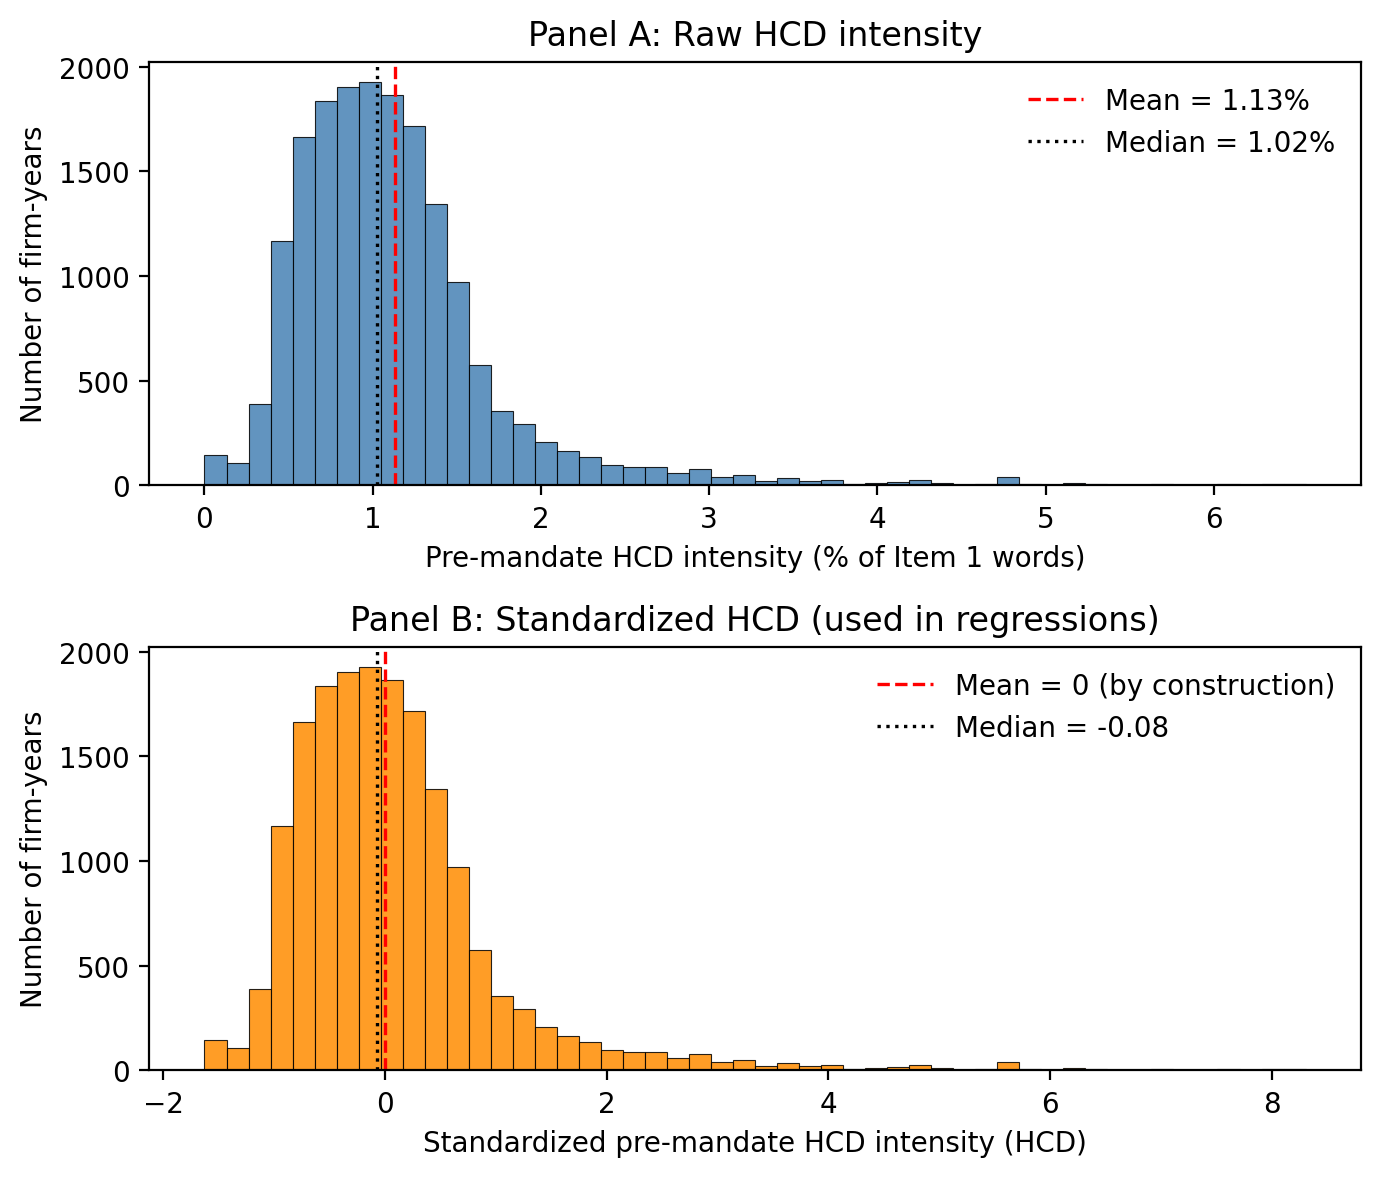
\includegraphics[width=0.85\textwidth]{fig_hcd_distribution.png}
\caption{Distribution of Pre-Mandate Human Capital Disclosure (HCD) Intensity}
\label{fig:hcd}
\begin{minipage}{0.85\textwidth}
\footnotesize
\textit{Notes:} The figure shows the distribution of the firm-level pre-mandate HCD intensity measure used in the empirical analysis. Pre-mandate HCD intensity is the firm-level mean of Item~1 HCD intensity over FY2015--FY2019, where Item~1 HCD intensity is the count of HCD lexicon terms in Item~1 normalized by the Item~1 word count. The lexicon is from \citet{demers_al2024}. The top panel shows the raw (unstandardized) intensity in percentage points. The bottom panel shows the standardized measure used in the regressions, which has mean zero and unit standard deviation across firms in the regression sample. The sample is the strict regression sample of 17,544 firm-years from 3,248 unique firms over FY2017--FY2023. All values are winsorized at the 1st and 99th percentiles.
\end{minipage}
\end{figure}

\end{document}
